\documentclass[journal,12pt,twocolumn]{IEEEtran}
%
\usepackage{setspace}
\usepackage{gensymb}
\singlespacing
\usepackage[cmex10]{amsmath}
\usepackage{siunitx}
\usepackage{amsthm}

\usepackage{mathrsfs}

\usepackage{txfonts}
\usepackage{stfloats}

\usepackage{steinmetz}
\usepackage{cite}
\usepackage{cases}
\usepackage{subfig}
\usepackage{longtable}
\usepackage{multirow}
\usepackage{enumitem}
\usepackage{mathtools}
\usepackage{tikz}
\usepackage{circuitikz}
\usepackage{verbatim}
\usepackage{tfrupee}
\usepackage[breaklinks=true]{hyperref}
\usepackage{tkz-euclide} % loads  TikZ and tkz-base
\usetikzlibrary{calc,math}
\usetikzlibrary{fadings}
\usepackage{listings}
    \usepackage{color}                                            %%
    \usepackage{array}                                            %%
    \usepackage{longtable}                                        %%
    \usepackage{calc}                                             %%
    \usepackage{multirow}                                         %%
    \usepackage{hhline}                                           %%
    \usepackage{ifthen}                                           %%
  %optionally (for landscape tables embedded in another document): %%
    \usepackage{lscape}     
\usepackage{multicol}
\usepackage{chngcntr}
\DeclareMathOperator*{\Res}{Res}

\renewcommand\thesection{\arabic{section}}
\renewcommand\thesubsection{\thesection.\arabic{subsection}}
\renewcommand\thesubsubsection{\thesubsection.\arabic{subsubsection}}

\renewcommand\thesectiondis{\arabic{section}}
\renewcommand\thesubsectiondis{\thesectiondis.\arabic{subsection}}
\renewcommand\thesubsubsectiondis{\thesubsectiondis.\arabic{subsubsection}}

\hyphenation{op-tical net-works semi-conduc-tor}
\def\inputGnumericTable{}                                 %%

\lstset{
%language=C,
frame=single, 
breaklines=true,
columns=fullflexible
}
\begin{document}
%


\newtheorem{theorem}{Theorem}[section]
\newtheorem{problem}{Problem}
\newtheorem{proposition}{Proposition}[section]
\newtheorem{lemma}{Lemma}[section]
\newtheorem{corollary}[theorem]{Corollary}
\newtheorem{example}{Example}[section]
\newtheorem{definition}[problem]{Definition}
\newcommand{\BEQA}{\begin{eqnarray}}
\newcommand{\EEQA}{\end{eqnarray}}
\newcommand{\define}{\stackrel{\triangle}{=}}
\bibliographystyle{IEEEtran}
\providecommand{\mbf}{\mathbf}
\providecommand{\pr}[1]{\ensuremath{\Pr\left(#1\right)}}
\providecommand{\qfunc}[1]{\ensuremath{Q\left(#1\right)}}
\providecommand{\sbrak}[1]{\ensuremath{{}\left[#1\right]}}
\providecommand{\lsbrak}[1]{\ensuremath{{}\left[#1\right.}}
\providecommand{\rsbrak}[1]{\ensuremath{{}\left.#1\right]}}
\providecommand{\brak}[1]{\ensuremath{\left(#1\right)}}
\providecommand{\lbrak}[1]{\ensuremath{\left(#1\right.}}
\providecommand{\rbrak}[1]{\ensuremath{\left.#1\right)}}
\providecommand{\cbrak}[1]{\ensuremath{\left\{#1\right\}}}
\providecommand{\lcbrak}[1]{\ensuremath{\left\{#1\right.}}
\providecommand{\rcbrak}[1]{\ensuremath{\left.#1\right\}}}
\theoremstyle{remark}
\newtheorem{rem}{Remark}
\newcommand{\sgn}{\mathop{\mathrm{sgn}}}
\providecommand{\abs}[1]{\left\vert#1\right\vert}
\providecommand{\abs}[1]{\lvert#1\rvert} 
\providecommand{\res}[1]{\Res\displaylimits_{#1}} 
\providecommand{\norm}[1]{\left\lVert#1\right\rVert}
%\providecommand{\norm}[1]{\lVert#1\rVert}
\providecommand{\mtx}[1]{\mathbf{#1}}
\providecommand{\mean}[1]{E\left[ #1 \right]}
\providecommand{\fourier}{\overset{\mathcal{F}}{ \rightleftharpoons}}
%\providecommand{\hilbert}{\overset{\mathcal{H}}{ \rightleftharpoons}}
\providecommand{\system}{\overset{\mathcal{H}}{ \longleftrightarrow}}
	%\newcommand{\solution}[2]{\textbf{Solution:}{#1}}
\newcommand{\solution}{\noindent \textbf{Solution: }}
\newcommand{\cosec}{\,\text{cosec}\,}
\providecommand{\dec}[2]{\ensuremath{\overset{#1}{\underset{#2}{\gtrless}}}}
\newcommand{\myvec}[1]{\ensuremath{\begin{pmatrix}#1\end{pmatrix}}}
\newcommand{\mydet}[1]{\ensuremath{\begin{vmatrix}#1\end{vmatrix}}}
\numberwithin{equation}{subsection}
\makeatletter
\@addtoreset{figure}{problem}
\makeatother
\let\StandardTheFigure\thefigure
\let\vec\mathbf
\renewcommand{\thefigure}{\theproblem}
\def\putbox#1#2#3{\makebox[0in][l]{\makebox[#1][l]{}\raisebox{\baselineskip}[0in][0in]{\raisebox{#2}[0in][0in]{#3}}}}
     \def\rightbox#1{\makebox[0in][r]{#1}}
     \def\centbox#1{\makebox[0in]{#1}}
     \def\topbox#1{\raisebox{-\baselineskip}[0in][0in]{#1}}
     \def\midbox#1{\raisebox{-0.5\baselineskip}[0in][0in]{#1}}
\vspace{3cm}
\title{ASSIGNMENT-3}
\author{T.Naveena}
\maketitle
\newpage
\bigskip
\renewcommand{\thefigure}{\theenumi}
\renewcommand{\thetable}{\theenumi}
Download all python codes from 
\begin{lstlisting}
https://github.com/ThurpuNaveena/ASSIGNMENT-3/tree/main/CODES
\end{lstlisting}
%
and latex-tikz codes from 
%
\begin{lstlisting}
https://github.com/ThurpuNaveena/ASSIGNMENT-3/tree/main
\end{lstlisting}
%
%
\section{QUESTION No-2.36 (a) (Linear forms)}
Find the equation of the planes that passes through three points 
\myvec{1\\1\\-1},\myvec{6\\4\\-5},\myvec{-4\\-2\\3}
%
\section{Solution}
\begin{align}
\vec{R} = \myvec{1\\1\\-1},\vec{S} = \myvec{6\\4\\-5} \text{and} \vec{T} = \myvec{-4\\-2\\3}
\end{align}
\\ If the equation of the plane is given by
\begin{align}
\vec{n}^T\vec{x} = 1
\end{align}
\begin{align}
\myvec{1&1&-1 \\ 6&4&-5 \\ -4&-2&3} \vec{n} &= \myvec{1\\1\\1}
\end{align}
Row reducing the augmented matrix, 
\begin{align}
\myvec{1 & 1 & -1 & 1\\6 & 4 & -5 & 1\\-4 & -2 & 3 & 1}
\xleftrightarrow {R_2\rightarrow 
R_2-6R_1}\myvec{1 & 1 & -1 & 1\\0 & -2 & 1 & -5\\-4 & -2 & 3 & 1}
\\
\xleftrightarrow{R_3\rightarrow R_3+4R_1}\myvec{1 & 1 & -1 & 1\\0 & -2 & 1 & -5\\0 & 2 & -1 & 5}
\\
\xleftrightarrow{R_2\rightarrow\frac{-R_2}{3}}\myvec{1 & 1 & -1 & 1\\0 & 1 & \frac{-1}{2} & \frac{5}{2}\\0 & 2 & -1 & 5}
\\
\xleftrightarrow{R_1\rightarrow{R_1-R_2}}\myvec{1 & 0 & \frac{-1}{2} & \frac{-3}{2}\\0 & 1 & \frac{-1}{2} & \frac{5}{2}\\0 & 2 & -1 & 5}
\\
\xleftrightarrow{R_3\rightarrow{R_3-2R_2}}\myvec{1 & 0 & \frac{-1}{2} & \frac{-3}{2}\\0 & 1 & \frac{-1}{2} & \frac{5}{2}\\0 & 0 & 0 & 0}
\\
\myvec{1 & 0 & -0.5 & -1.5\\0 & 1 & -0.5 & 2.5\\0 & 0 & 0 & 0}
\end{align}
Number of Non zero row =2.
Rank of Matrix =2
For the linear equation to have infinite solution.
Rank(coefficient matrix) = Rank(Augmented matrix)and both not equal to  Rank (Full matrix)
\begin{align}
\myvec{1 & 1 & -1\\6 & 4 & -5\\-4 & -2 & 3}
\end{align}
Row reduced matrix
\begin{align}
\myvec{1 & 0 & -0.5\\0 & 1 & -0.5\\0 & 0 & 0}
\end{align}
Rank of matrix =3

Rank of coefficient matrix = 0

since the given matrix has infinite solutions,there are infinitely many planes passing through the points which means that they lie on a straight line.

 Equation of the line
\begin{align}
\vec{A} = \myvec{1 \\ 6 \\ -4} , \vec{B} = \myvec{1 \\ 4 \\ -2}
\\
\vec{x} = \vec{A}+\lambda\brak{{\vec{B}-\vec{A}}}
\\
\vec{x} &= \myvec{1 \\ 6 \\ -4}+\lambda\myvec{0 \\ -2 \\2}
\end{align}
\numberwithin{figure}{section}
\begin{figure}[ht]
\centering
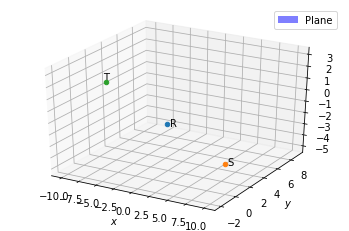
\includegraphics[width=\columnwidth]{figure.png}
\caption{plot of the line}
\label{Plot of the line}
\end{figure}
\end{document}

